\renewcommand*{\arraystretch}{1.1}

\subsection*{Interactive / update / 7}
\label{section:interactive-update-07}

% change \emph{} to use sans-serif font
\let\oldemph\emph
\renewcommand{\emph}[1]{{\footnotesize \sf #1}}

\renewcommand{\currentQueryCard}{7}
\marginpar{
	\raggedleft
	\vspace{0.22ex}

	\queryRefCard{interactive-update-01}{IU}{1}\\
	\queryRefCard{interactive-update-02}{IU}{2}\\
	\queryRefCard{interactive-update-03}{IU}{3}\\
	\queryRefCard{interactive-update-04}{IU}{4}\\
	\queryRefCard{interactive-update-05}{IU}{5}\\
	\queryRefCard{interactive-update-06}{IU}{6}\\
	\queryRefCard{interactive-update-07}{IU}{7}\\
	\queryRefCard{interactive-update-08}{IU}{8}\\
}


\noindent\begin{tabularx}{\queryCardWidth}{|>{\queryPropertyCell}p{\queryPropertyCellWidth}|X|}
	\hline
	query & Interactive / update / 7 \\ \hline
%
	title & Add Comment \\ \hline
%
	pattern & \multicolumn{1}{c|}{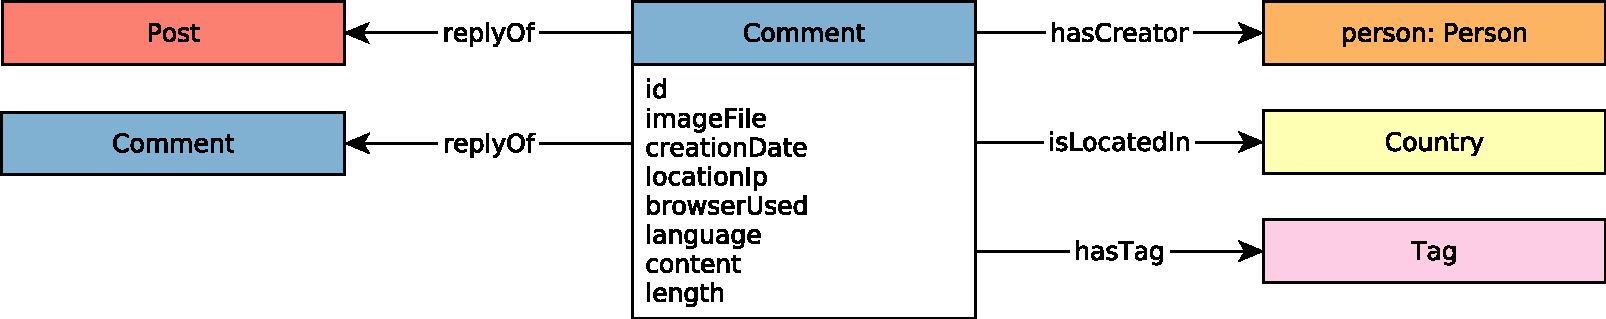
\includegraphics[scale=\patternscale,margin=0cm .2cm]{patterns/interactive-update-07}} \\ \hline
%
	desc. & Add a Comment replying to a Post/Comment to the social network.
 \\ \hline
%
	
		params &
		\innerCardVSpace{\begin{tabularx}{\attributeCardWidth}{|>{\paramNumberCell}c|>{\varNameCell}M|>{\typeCell}m{\typeWidth}|Y|} \hline
		$\mathsf{1}$ & Comment.id
 & ID
 &  \\ \hline
		$\mathsf{2}$ & Comment.creationDate
 & DateTime
 &  \\ \hline
		$\mathsf{3}$ & Comment.locationIp
 & String
 &  \\ \hline
		$\mathsf{4}$ & Comment.browserUsed
 & String
 &  \\ \hline
		$\mathsf{5}$ & Comment.content
 & Text
 &  \\ \hline
		$\mathsf{6}$ & Comment.length
 & 32-bit Integer
 &  \\ \hline
		$\mathsf{7}$ & Comment-hasCreator-\textgreater{}Person.id
 & ID
 &  \\ \hline
		$\mathsf{8}$ & Comment-isLocatedIn-\textgreater{}Country.id
 & ID
 &  \\ \hline
		$\mathsf{9}$ & Comment-replyOf-\textgreater{}Post.id
 & ID
 & \(-1\) if the comment is a reply of a comment
 \\ \hline
		$\mathsf{10}$ & Comment-replyOf-\textgreater{}Comment.id
 & ID
 & \(-1\) if the comment is a reply of a post
 \\ \hline
		$\mathsf{11}$ & \{Comment-hasTag-\textgreater{}Tag.id\}
 & \{ID\}
 &  \\ \hline
		\end{tabularx}}\innerCardVSpace \\ \hline
	
%
	
%
	%
	%
	%
	%
\end{tabularx}
\queryCardVSpace

% change \emph back to the old one
\renewcommand{\emph}[1]{\oldemph{#1}}